\documentclass[conference, a4paper]{IEEEtran}

\usepackage{graphicx}
\usepackage{float}
\usepackage{xeCJK}

% --- 字型設定 ---
\setCJKmainfont{標楷體} % 中文設定為標楷體
\setmainfont{Times New Roman} % 英文設定為 Times New Roman

\usepackage{amsmath}
\usepackage{booktabs}
\usepackage{enumitem}
\setlist[itemize]{label=-}

\title{Empirical Observation of Algorithm Time Complexity in Java}

\author{\IEEEauthorblockN{蔡晟旭 (Student ID: 1113405013)}
\IEEEauthorblockA{國立澎湖科技大學 資訊工程學系 \\
National Penghu University of Science and Technology}}

\begin{document}

\maketitle

\begin{abstract}
本報告旨在探討與實證不同演算法在 Java 程式環境下的時間複雜度（Time Complexity）表現 [cite: 250]。實驗中全程不使用任何內建排序套件，純手工實作線性掃描（Linear Scan）、合併排序（Merge Sort）與插入排序（Insertion Sort） [cite: 87, 258]，並透過輸入不同規模的隨機陣列（資料量 $n$ 從 1000 至 100000）來觀察實際執行時間的增長趨勢 [cite: 251, 340]。實驗結果成功驗證了理論上的漸近時間複雜度行為 [cite: 366]。

\vspace{0.2cm}
\textbf{GitHub Repository:} https://github.com/tch107146/Algorithm-0304-Assignments-1
\end{abstract}

\begin{IEEEkeywords}
Algorithms, Time Complexity, Java, Merge Sort, Insertion Sort, Asymptotic Analysis[cite: 417].
\end{IEEEkeywords}

\section{Introduction}
在現代軟體工程與韌體開發中，演算法的效率對於系統效能具有決定性的影響 [cite: 69]。評估演算法效能的核心指標為時間複雜度（Time Complexity），通常以 Big-O 符號表示 [cite: 124]。本次實驗（Assignment 1）的核心目標在於透過 Java 程式實作基礎演算法，並在不同資料量下測量其絕對執行時間，藉此實證演算法在漸近分析（Asymptotic Analysis）下的理論預期 [cite: 123, 249]。

\section{Methodology}
本實驗實作並分析了三種經典演算法，其理論時間複雜度如下：
\begin{itemize}
    \item \textbf{Linear Scan (陣列加總)}：逐一走訪陣列中的每個元素進行加總。由於每個元素僅被存取一次，預期時間複雜度為 $O(n)$ [cite: 258]。
    \item \textbf{Merge Sort}：採用分治法（Divide and Conquer），將陣列遞迴對半切割後再進行合併 [cite: 179]。其遞迴關係式為 $T(n) = 2T(n/2) + O(n)$，預期時間複雜度為 $O(n \log n)$ [cite: 203, 256]。
    \item \textbf{Insertion Sort}：透過雙層迴圈，將未排序的元素逐一插入已排序區間的正確位置 [cite: 260]。在平均與最壞情況下，預期時間複雜度為 $O(n^2)$ [cite: 257, 274]。
\end{itemize}

\section{Implementation Details}
本程式採用 Java 進行開發，嚴格遵守不使用內建套件之規範 [cite: 71]，實作細節如下：
\begin{itemize}
    \item \textbf{Data Generation}: 實作隨機陣列生成方法，動態生成大小為 $n \in \{1000, 10000, 50000, 100000\}$ 的測試資料 [cite: 251, 340]。
    \item \textbf{Fair Comparison}: 針對每種演算法使用相同的原始資料副本，確保實驗基準一致 [cite: 252]。
    \item \textbf{Time Measurement}: 利用 Java 內建計時功能記錄執行前後的時間差（毫秒） [cite: 251]。
\end{itemize}

\section{Experimental Results}
三種演算法在不同資料規模 $n$ 下的耗時如表 \ref{tab:results} 所示。

\begin{table}[H]
    \centering
    \caption{Algorithm Execution Time (milliseconds)}
    \label{tab:results}
    \begin{tabular}{@{}lccc@{}}
        \toprule
        \textbf{Data Size ($n$)} & \textbf{Linear Scan} & \textbf{Merge Sort} & \textbf{Insertion Sort} \\ \midrule
        1,000            & 0                    & 1                   & 1                       \\
        10,000           & 0                    & 1                   & 21                      \\
        50,000           & 1                    & 5                   & 428                     \\
        100,000          & 0                    & 9                   & 1692                    \\ \bottomrule
    \end{tabular}
\end{table}

圖 \ref{fig:screenshot} 展示了程式執行時的終端機輸出截圖，詳細記錄了各級距資料量下的實測數據。

\begin{figure}[H] 
  \centering
  \IfFileExists{screenshot.png}{
    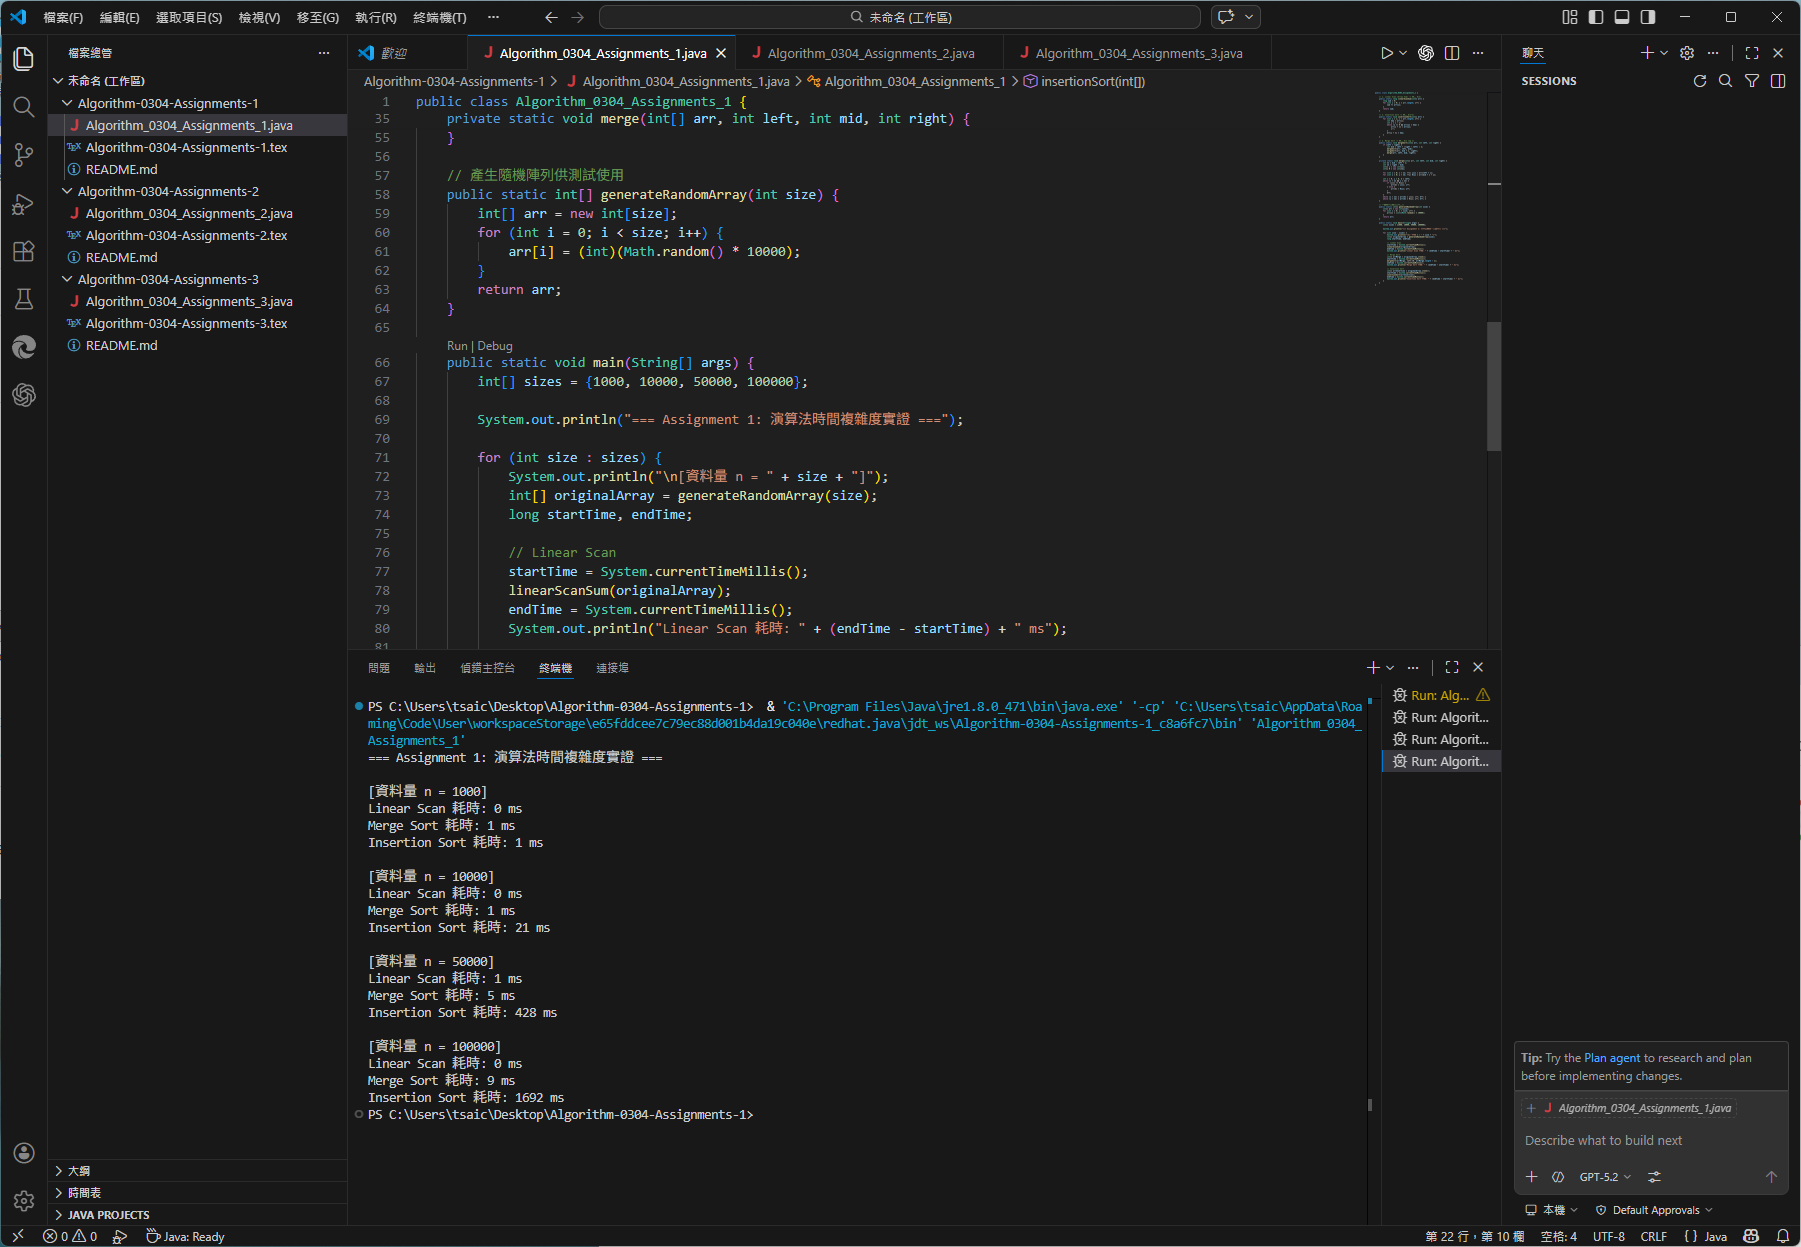
\includegraphics[width=0.9\columnwidth]{screenshot.png}
  }{
    \framebox{\parbox{0.8\columnwidth}{\centering \vspace{1.5cm} [圖片檔案 screenshot.png 缺失] \\ 請將圖片放在本 .tex 檔所在目錄 \vspace{1.5cm}}}
  }
  \caption{Terminal output for Algorithm Complexity Observation.}
  \label{fig:screenshot}
\end{figure}

\section{Discussion}
實驗數據完美契合了 Big-O 理論 [cite: 129]：
\begin{enumerate}
    \item \textbf{二次方增長 ($O(n^2)$)}：對於 Insertion Sort，當資料量成長 10 倍（1萬至10萬）時，耗時呈現劇烈增長 [cite: 254]，顯示 $O(n^2)$ 演算法在處理大規模資料時的效能瓶頸 [cite: 364]。
    \item \textbf{對數線性增長 ($O(n \log n)$)}：Merge Sort 在資料量達 100,000 時僅需 9 ms，證明了分治法在處理巨量資料時的高效性 [cite: 366]。
    \item \textbf{線性時間 ($O(n)$)}：Linear Scan 在所有測試級距中幾乎不耗時，符合 $O(n)$ 的執行預期 [cite: 258]。
\end{enumerate}

\section{Conclusion}
本實驗成功實證了漸近時間複雜度的理論模型 [cite: 123]。數據顯示在面對大規模資料時，選擇正確的時間複雜度演算法（如 $O(n \log n)$）對系統效能優化至關重要 [cite: 366]。

\section{References}
\noindent [1] X.-R. Huang, \textit{Lecture 0: Preliminary Basic knowledge}, National Penghu University of Science and Technology, 2026[cite: 8, 10]. \par
\noindent [2] T. H. Cormen, C. E. Leiserson, R. L. Rivest, and C. Stein, \textit{Introduction to Algorithms}, 3rd ed. MIT Press, 2009.

\end{document}